\documentclass[11pt]{article}

\usepackage[margin=0.82in]{geometry}
\usepackage[T1]{fontenc}
\usepackage[utf8]{inputenc}
\usepackage{lmodern}
\usepackage{microtype}
\usepackage{amsmath,amssymb,mathtools}
\usepackage{booktabs}
\usepackage{array}
\usepackage{tabularx}
\usepackage{longtable}
\usepackage{graphicx}
\usepackage{xcolor}
\usepackage{enumitem}
\usepackage{caption}
\usepackage{float}
\usepackage{placeins}
\usepackage{hyperref}

\definecolor{navy}{HTML}{17365D}
\definecolor{blue}{HTML}{DCE6F1}
\definecolor{green}{HTML}{E2F0D9}
\definecolor{orange}{HTML}{FCE4D6}
\definecolor{graybox}{HTML}{F2F2F2}

\hypersetup{
  colorlinks=true,
  linkcolor=navy,
  citecolor=navy,
  urlcolor=navy,
  pdftitle={Food-Composition Foundation Evidence under Explicit Dependency Masking},
  pdfauthor={Representation Model Study}
}

\graphicspath{{figures/}}
\setlist[itemize]{leftmargin=1.5em,itemsep=2pt,topsep=4pt}
\setlist[enumerate]{leftmargin=1.7em,itemsep=2pt,topsep=4pt}
\setlength{\tabcolsep}{5pt}
\renewcommand{\arraystretch}{1.12}
\newcommand{\foodtoken}{\texttt{[FOOD]}}
\newcommand{\SLMAE}{\operatorname{SLMAE}}
\newcommand{\SLRMSE}{\operatorname{SLRMSE}}
\newcommand{\RawMAE}{\operatorname{RawMAE}}

\title{\textbf{Food-Composition Foundation Evidence\\under Explicit Dependency Masking}\\
\large Revised English Report: External Transfer, Sparse Completion, and Sensitivity}
\author{Representation Model Study}
\date{28 October 2026}

\begin{document}
\maketitle

\begin{abstract}
This report evaluates a food-composition completion model trained without food names, database identifiers, food-family labels, or profile identifiers. The dependency mask is part of both training and inference: for each target axis, the target and its registered directed ancestors and descendants are hidden, while siblings remain visible. The validation-selected V5+CCE model achieves the lowest complete-test macro scaled-log MAE among the formal methods (0.3016). On a Taiwan TFDA external panel it also gives the best strict zero-shot score (0.1922). On a fixed name-novel Taiwan test, frozen V5+CCE scores 0.2000, compared with 0.4551/0.3266/0.2430 for Taiwan-only RF fits and 0.5287/0.3262/0.2369 for Taiwan-only XGBoost fits at 8/32/128 profiles. With only 5--20 visible composition values, V5+CCE also outperforms RF, XGBoost, and KNN. An FAO/INFOODS-based group sensitivity audit finds larger average within-group than between-group prediction responses. A stricter dependency-family exposure ablation is negative: exposing normally hidden relatives worsens error, and their perturbation does not move predictions more than matched unrelated controls. The latter result supports retaining the mask but does not establish that the trained model has learned unusually strong parent--component dependence.
\end{abstract}

\section{Scope and Shared Protocol}

\subsection{Task and data restrictions}

For profile $i$, let $C_i$ be the visible composition axes and let $t$ be a queried target. The predictor receives the unordered numerical context
\begin{equation}
  \mathcal{C}_{i,t}=\{(a,y_{i,a}):a\in C_i,\ y_{i,a}\text{ observed and permitted by the target mask}\}
\end{equation}
and returns $\hat y_{i,t}$. The study contains 252 composition axes, of which 187 are supervised targets. Missing values are absent tokens; an explicit zero is a valid observed value. Food name, source/database identity, semantic food category, legacy family label, exact-name group, and profile index never enter any predictor.

The complete-test panel contains 659 profiles and 19,690 observed profile--axis jobs spanning all 187 supervised axes. Normalization uses training data only. For axis $a$,
\begin{align}
  s_a &= \operatorname{median}\{y_{i,a}:y_{i,a}>0,\ y_{i,a}\text{ observed in training}\},\\
  z_{i,a} &= \log\left(1+\frac{y_{i,a}}{s_a}\right),\\
  \hat y_{i,a} &= s_a\left[\exp\bigl(\max(\hat z_{i,a},0)\bigr)-1\right].
\end{align}

For scaled-log error $d_{i,a}=\hat z_{i,a}-z_{i,a}$ and $N_a$ scored jobs on axis $a$, the three macro metrics are
\begin{align}
\SLMAE &= \frac{1}{187}\sum_a\frac{1}{N_a}\sum_i|d_{i,a}|,\\
\SLRMSE &= \frac{1}{187}\sum_a\sqrt{\frac{1}{N_a}\sum_i d_{i,a}^2},\\
\RawMAE &= \frac{1}{187}\sum_a\frac{1}{N_a}\sum_i|\hat y_{i,a}-y_{i,a}|.
\end{align}
Lower is better. The scaled-log metrics give every axis equal macro weight after robust per-axis scaling; raw MAE retains the original concentration scale.

\subsection{Explicit dependency mask}

The mask graph contains only totals, components, subtotals, and structural members supported by FAO/INFOODS component definitions \cite{infoodstags}. It contains 37 directed relations over 44 axes. Of 187 supervised targets, 144 are unregistered singletons. For target $t$, the hidden set is
\begin{equation}
  M(t)=\{t\}\cup\operatorname{Ancestors}(t)\cup\operatorname{Descendants}(t).
\end{equation}
Sibling axes remain visible. The legacy broad \texttt{mask\_family} field is unused. Every training task applies this policy before batching, and the same policy is used for validation, complete test, Taiwan transfer, sparse completion, and sensitivity. The checkpoint records the mask-policy hash.

\subsection{V5+CCE model}

V5+CCE uses three Transformer layers, hidden dimension 192, six attention heads, ReGLU feed-forward width 256, full bidirectional attention, and ordered axis-pair attention bias. V5 executes the same Transformer twice. The first pass produces target predictions and a contextual \foodtoken{} state $h_{\mathrm{food}}^{(1)}$. The second pass replaces the initial \foodtoken{} vector with $\operatorname{stopgrad}(h_{\mathrm{food}}^{(1)})$ and produces the official prediction. CCE adds a contrastive objective between two dropout views of the first-pass \foodtoken{} representation, following the contrastive cell-embedding idea in scGPT \cite{scgpt}. Dropout and the CCE loss are disabled at inference.

\subsection{Complete-test benchmark}

\begin{table}[H]
\centering
\caption{Complete-test results under the explicit dependency mask. All 187 target axes are macro averaged.}
\label{tab:complete}
\begin{tabular}{@{}lrrr@{}}
\toprule
Method & Scaled-log MAE & Scaled-log RMSE & Raw MAE \\
\midrule
\textbf{V5+CCE} & \textbf{0.3016} & 0.4910 & 0.3137 \\
XGBoost & 0.3270 & \textbf{0.4825} & \textbf{0.2624} \\
RF & 0.3322 & 0.4841 & 0.2838 \\
KNN & 0.4047 & 0.5937 & 0.4729 \\
\bottomrule
\end{tabular}
\end{table}

V5+CCE is best on the primary scale-balanced typical-error metric. XGBoost is best on raw MAE and scaled-log RMSE, so no method dominates every error definition. The underlying values are provided in \path{tables/complete_test_model_metrics.csv}.

\section{Representation UMAP: Food Category and Database}

The first-pass V5+CCE \foodtoken{} representation is extracted for 4,000 validation profiles. UMAP \cite{umap} is fitted only for visualization; category and database labels are used for colouring and never for training or checkpoint selection. Figure~\ref{fig:umap} contains only the requested food-category and database views.

\begin{figure}[H]
\centering
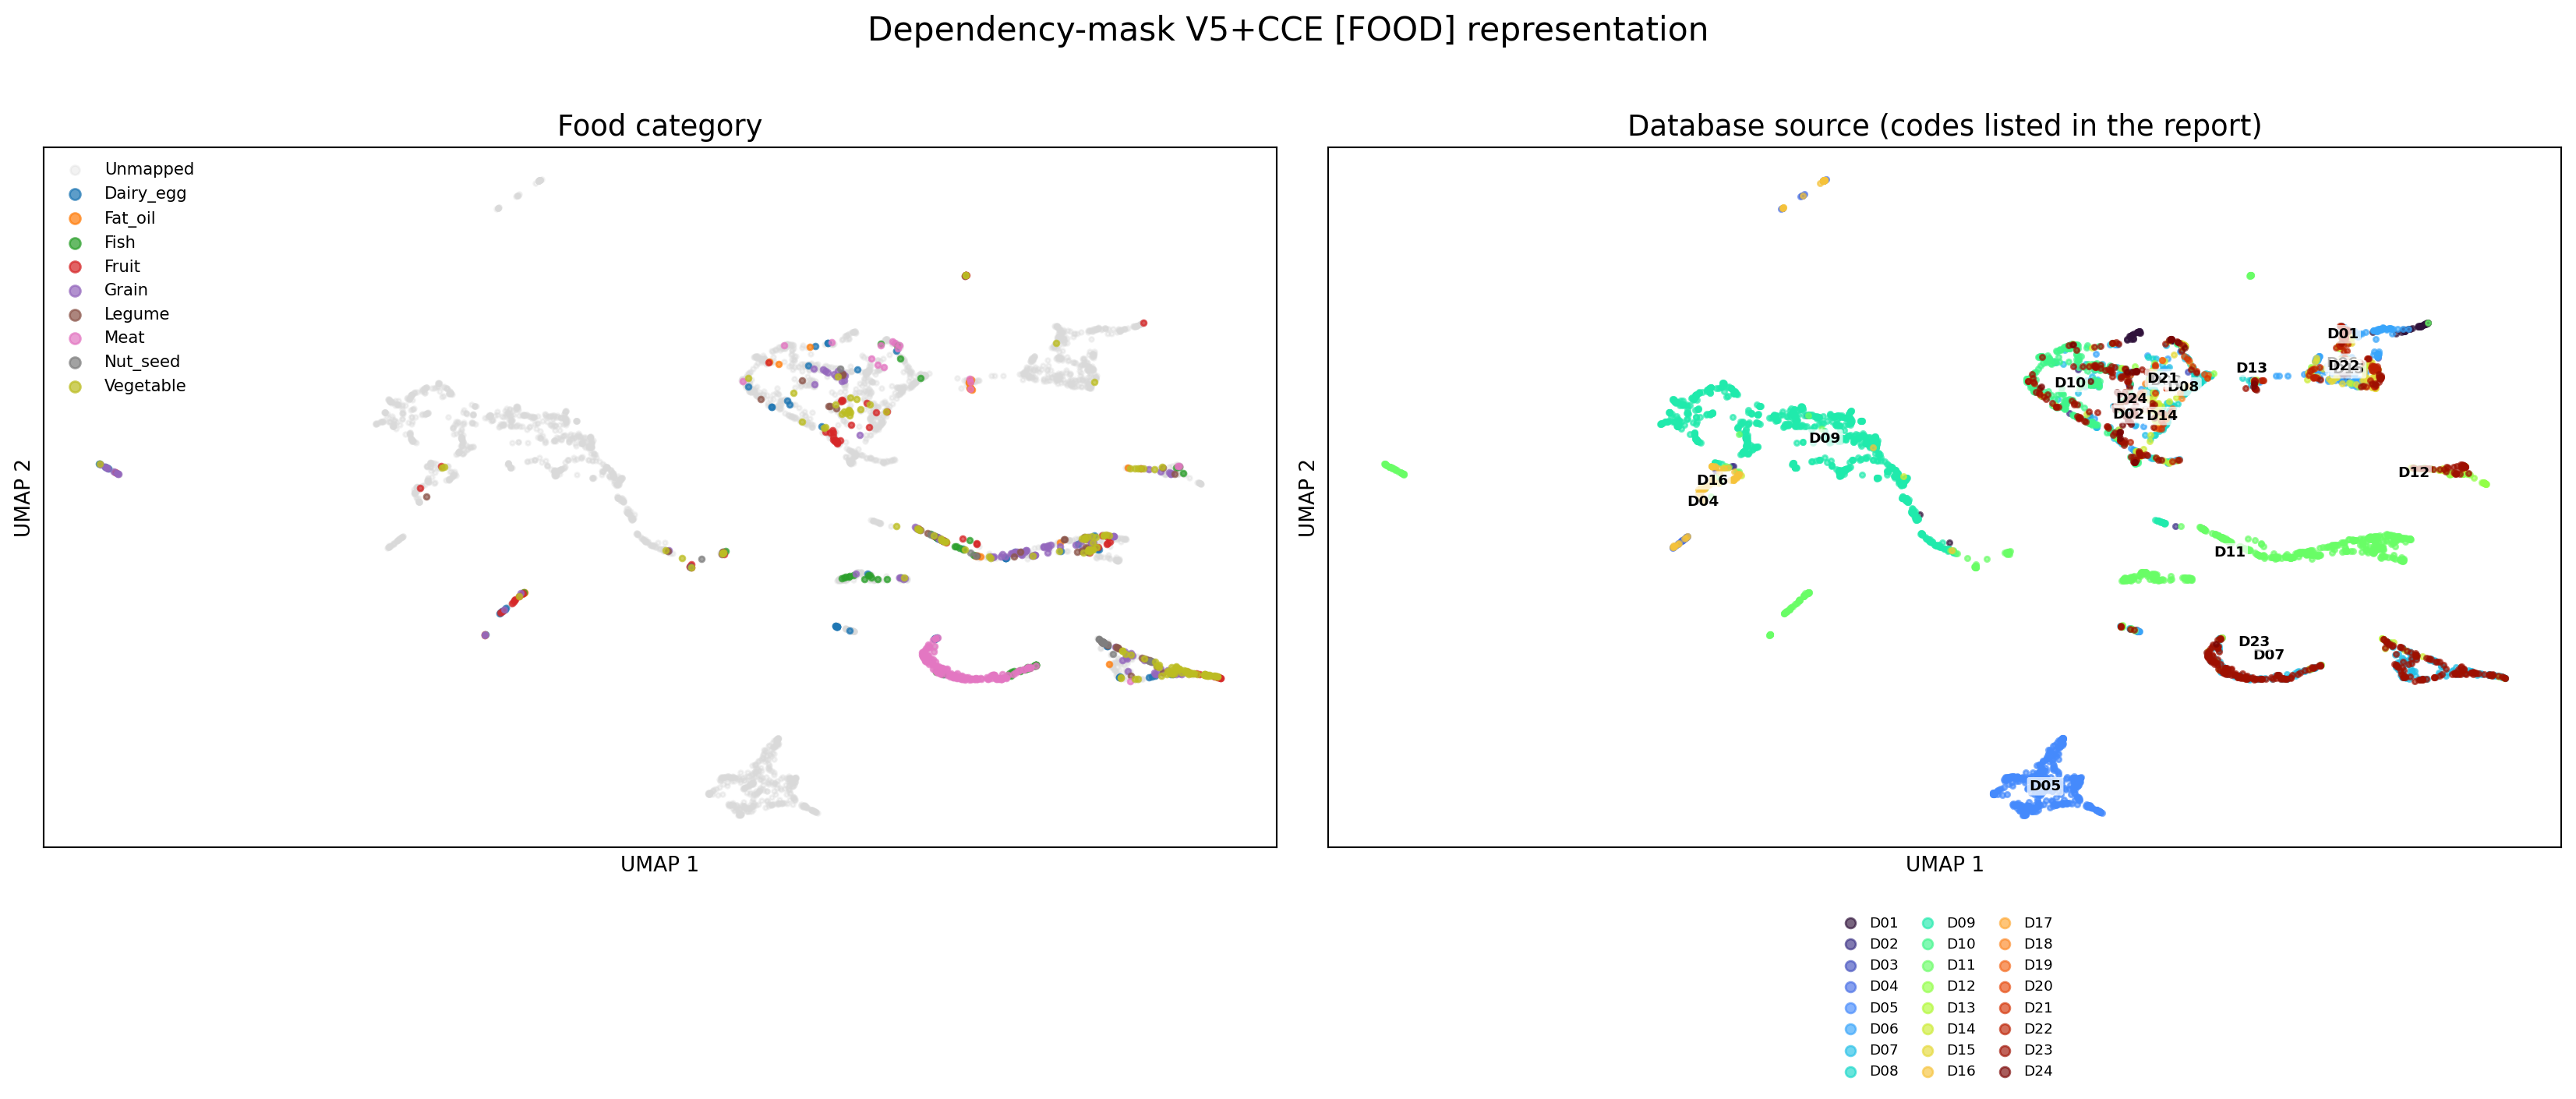
\includegraphics[width=\textwidth]{umap_food_category_database.png}
\caption{UMAP of V5+CCE \foodtoken{} representations. Unmapped food categories are grey. Database labels D01--D24 are expanded in Table~\ref{tab:db}.}
\label{fig:umap}
\end{figure}

\begin{table}[H]
\centering
\caption{Food-category probe metrics. Labels are used only after representation extraction.}
\begin{tabular}{@{}lrrr@{}}
\toprule
Representation & Macro purity@10 & Macro-F1 & Balanced accuracy \\
\midrule
Values + visibility mask & 0.7563 & 0.8614 & 0.8598 \\
V4 & 0.6424 & 0.7296 & 0.7505 \\
V5 & 0.6767 & 0.7592 & 0.7814 \\
V5+CCE & 0.6973 & 0.7895 & 0.8096 \\
\bottomrule
\end{tabular}
\end{table}

V5+CCE is more category-structured than V4 and V5, but the original numerical values plus visibility indicators remain more category-informative. Missingness alone reaches approximately 0.971 database-source balanced accuracy. Database separation is therefore materially confounded by source-specific coverage and should not be interpreted as pure food semantics.

\begin{longtable}{@{}>{\raggedright\arraybackslash}p{0.08\textwidth}>{\raggedright\arraybackslash}p{0.25\textwidth}>{\raggedright\arraybackslash}p{0.51\textwidth}r@{}}
\caption{Database codes used in Figure~\ref{fig:umap}. The final column is the number of profiles in the plotted UMAP sample.}\label{tab:db}\\
\toprule
Code & Source key & Database & $n$ \\
\midrule
\endfirsthead
\multicolumn{4}{c}{\tablename\ \thetable\ (continued)}\\
\toprule
Code & Source key & Database & $n$ \\
\midrule
\endhead
\midrule
\multicolumn{4}{r}{Continued on next page}\\
\endfoot
\bottomrule
\endlastfoot
D01 & afcd & Australian Food Composition Database & 107 \\
D02 & anfood\_2\_0 & FAO/INFOODS AnFooD 2.0 & 22 \\
D03 & bangladesh\_fct\_2013 & Bangladesh Food Composition Table 2013 & 15 \\
D04 & biofoodcomp\_4\_0 & FAO/INFOODS BioFoodComp 4.0 & 51 \\
D05 & bls\_4\_0 & German Nutrient Database BLS 4.0 & 405 \\
D06 & ciqual & ANSES-Ciqual & 194 \\
D07 & cnf & Canadian Nutrient File & 326 \\
D08 & cofid & UK CoFID & 141 \\
D09 & efsa\_eu\_fcdb\_2013 & EFSA EU Food Composition Database & 830 \\
D10 & fndds & USDA FNDDS & 273 \\
D11 & foodb & FooDB & 622 \\
D12 & frida & Frida FoodData, Denmark & 79 \\
D13 & lesotho\_fct\_2006 & Lesotho Food Composition Table 2006 & 12 \\
D14 & mext\_japan\_2023 & Japan MEXT Food Composition Tables & 133 \\
D15 & norway & Norwegian Food Composition Database & 87 \\
D16 & phyfoodcomp\_1\_0 & FAO/INFOODS/IZiNCG PhyFoodComp 1.0 & 112 \\
D17 & smiling\_cambodia\_2013 & SMILING Cambodia FCT 2013 & 6 \\
D18 & smiling\_indonesia\_2013 & SMILING Indonesia FCT 2013 & 6 \\
D19 & smiling\_laos\_2013 & SMILING Laos FCT 2013 & 6 \\
D20 & smiling\_thailand\_2013 & SMILING Thailand FCT 2013 & 7 \\
D21 & smiling\_vietnam\_2013 & SMILING Vietnam FCT 2013 & 11 \\
D22 & swiss\_fcdb\_7\_1 & Swiss Food Composition Database 7.1 & 73 \\
D23 & usda\_sr\_legacy & USDA Standard Reference Legacy & 431 \\
D24 & wafct\_2019 & FAO/INFOODS West Africa FCT 2019 & 51 \\
\end{longtable}

\FloatBarrier
\section{Taiwan TFDA External Transfer}

\subsection{Strict zero-shot evaluation}

Taiwan data are excluded from pretraining, scale estimation, hyperparameter tuning, and checkpoint selection. The strict panel contains 2,212 foods, 128,470 food--axis jobs, and 80 axes. All methods apply the same dependency mask. Tree and neighbour baselines in this zero-shot comparison are fitted on the original source training partition.

\begin{figure}[H]
\centering
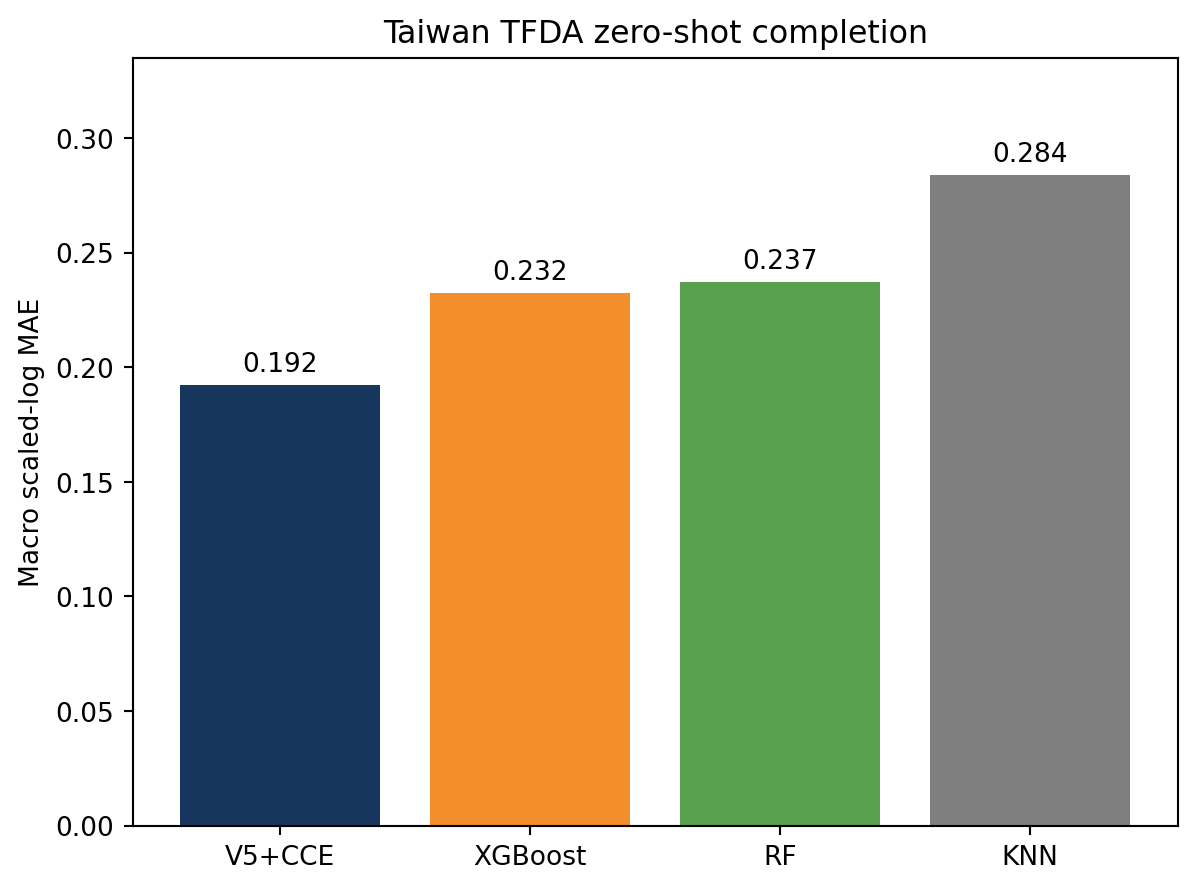
\includegraphics[width=0.78\textwidth]{taiwan_zero_shot.png}
\caption{Strict Taiwan zero-shot results. Lower scaled-log MAE is better.}
\label{fig:taiwan-zero}
\end{figure}

\begin{table}[H]
\centering
\caption{Strict Taiwan zero-shot metrics over 80 axes.}
\begin{tabular}{@{}lrrr@{}}
\toprule
Method & Scaled-log MAE & Scaled-log RMSE & Raw MAE \\
\midrule
\textbf{V5+CCE} & \textbf{0.1922} & \textbf{0.3703} & 0.3253 \\
XGBoost & 0.2324 & 0.3731 & \textbf{0.3185} \\
RF & 0.2370 & 0.3729 & 0.3332 \\
KNN & 0.2838 & 0.4519 & 0.4968 \\
\bottomrule
\end{tabular}
\end{table}

V5+CCE has the lowest strict-panel scaled-log MAE. The name-novel subset preserves the same ranking. Aggregate metrics and profile-paired bootstrap results are supplied in \path{tables/taiwan_zero_shot_metrics.csv} and \path{tables/taiwan_zero_shot_paired_bootstrap.csv}.

\subsection{Few-shot protocol}

Few-shot evaluation uses only Taiwan foods whose English names are absent from pretraining. A fixed 400-food test set is drawn once from the name-novel panel; it contains 23,944 jobs over all 80 evaluated axes. The remaining 1,389 foods form an adaptation pool. Three sampling seeds are used. For each seed, a missingness-only greedy set-cover step first guarantees that every evaluated axis has at least one label within the 8-profile subset; the remaining profiles are randomized. The subsets are nested: $8\subset32\subset128$. Neither nutrient values nor test errors influence selection.

V5+CCE remains completely frozen and does not consume any adaptation profile. RF and XGBoost are not continued from source-trained tree models: for every target axis, the unchanged formal estimator is fitted only on selected Taiwan profiles that have an observed label for that axis. Their 504-dimensional input contains 252 normalized values and 252 visibility indicators after target-specific dependency masking. This experiment is therefore a comparison of a frozen pretrained model with Taiwan-only few-shot tree fitting, rather than a comparison of three equally pretrained models.

\begin{figure}[H]
\centering
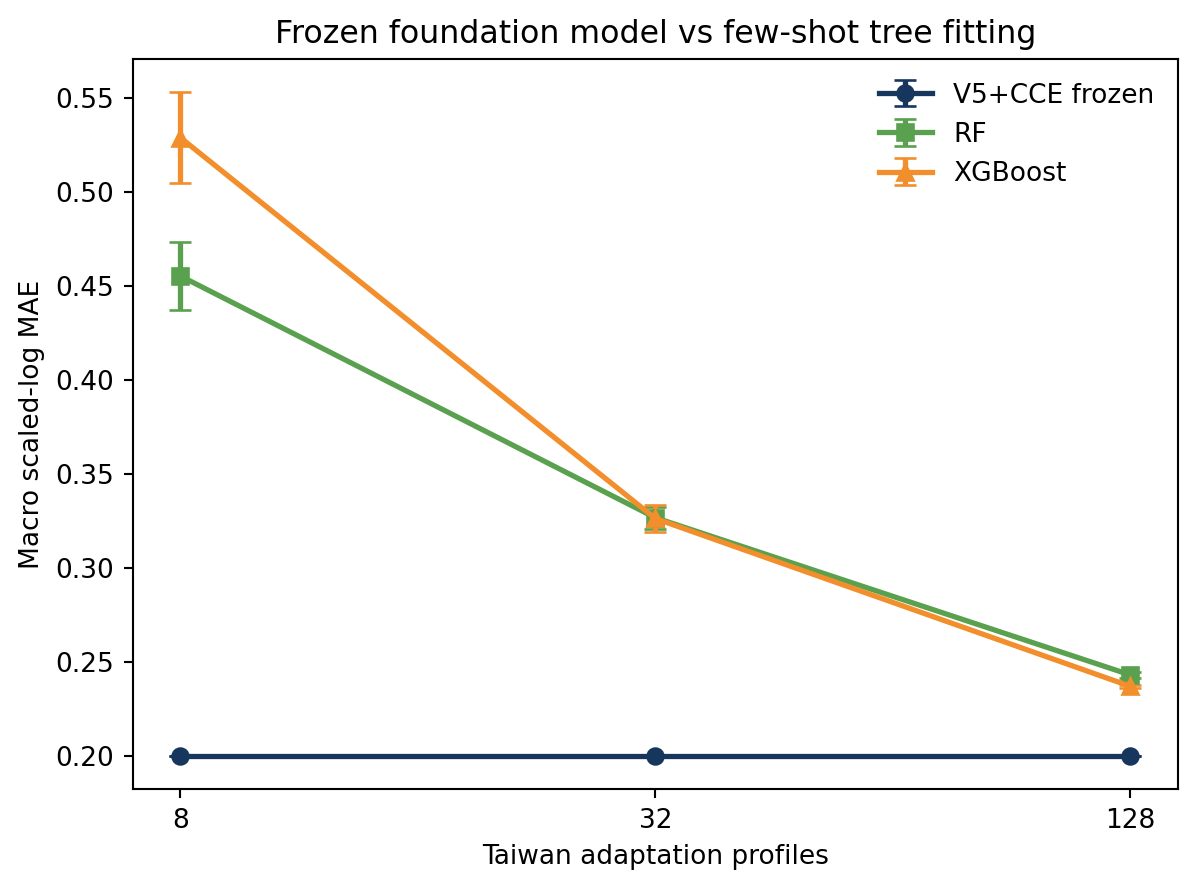
\includegraphics[width=0.82\textwidth]{taiwan_fewshot_curve.png}
\caption{Frozen V5+CCE versus Taiwan-only RF and XGBoost fits. Points for tree models are three-seed means; error bars show standard deviation.}
\label{fig:fewshot}
\end{figure}

\begin{table}[H]
\centering
\caption{Fixed-test Taiwan few-shot scaled-log MAE.}
\begin{tabular}{@{}lrrr@{}}
\toprule
Method & 8 profiles & 32 profiles & 128 profiles \\
\midrule
\textbf{V5+CCE frozen} & \textbf{0.2000} & \textbf{0.2000} & \textbf{0.2000} \\
RF & $0.4551\pm0.0179$ & $0.3266\pm0.0058$ & $0.2430\pm0.0017$ \\
XGBoost & $0.5287\pm0.0243$ & $0.3262\pm0.0074$ & $0.2369\pm0.0010$ \\
\bottomrule
\end{tabular}
\end{table}

Even with 128 local profiles, neither Taiwan-only tree fit reaches the frozen model. This supports external sample efficiency from source pretraining. It does not isolate architecture from the amount of source data, because only V5+CCE is pretrained in this particular comparison.

\FloatBarrier
\section{Completion with Few Visible Observations}

The sparse panel fixes 12 high-support validation targets and 200 jobs per target, for 2,400 jobs. Each job first applies the dependency mask and then retains 5, 10, 20, 40, or all remaining context values. Finite budgets use three repeats. The comparison contains only V5+CCE, RF, XGBoost, and KNN.

\begin{figure}[H]
\centering
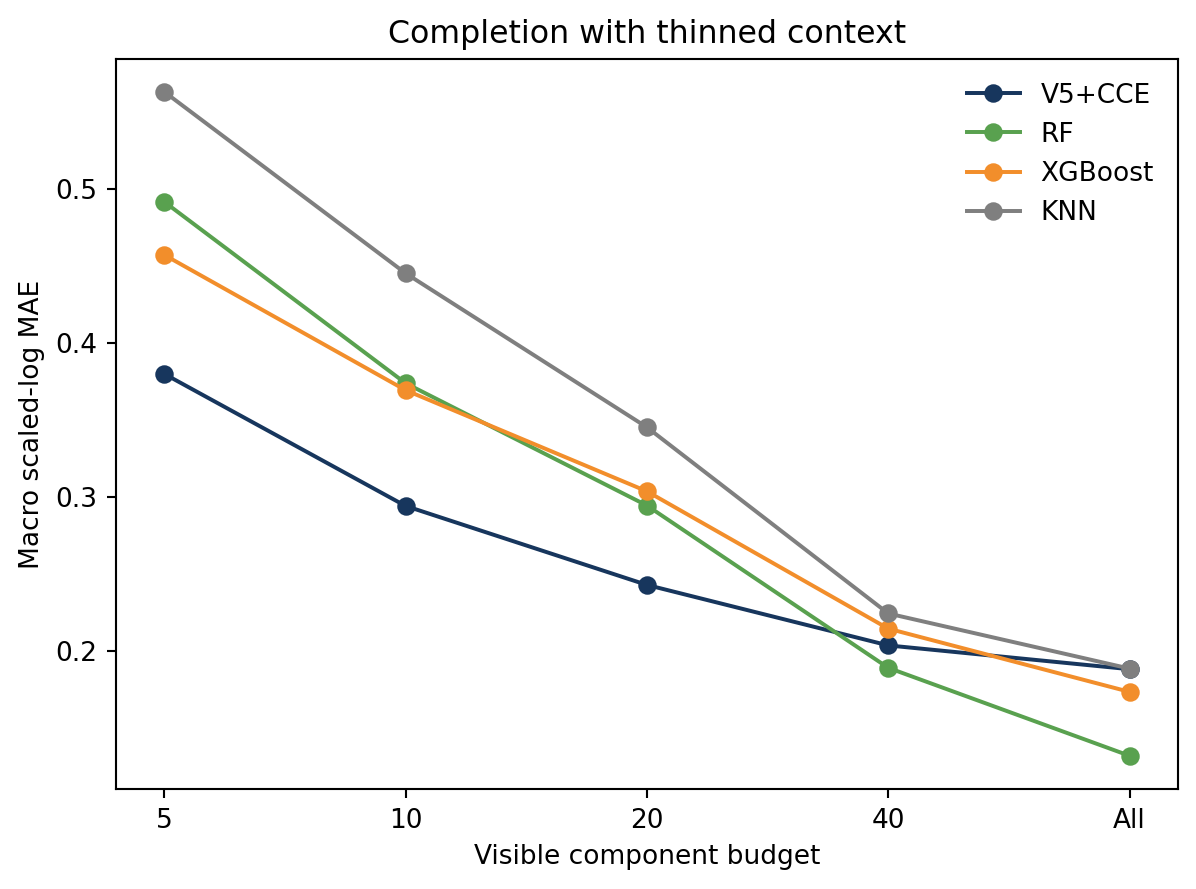
\includegraphics[width=0.82\textwidth]{sparse_observation_curve.png}
\caption{Macro scaled-log MAE as visible numerical context increases.}
\label{fig:sparse}
\end{figure}

\begin{table}[H]
\centering
\caption{Sparse-completion scaled-log MAE. Finite budgets are three-repeat means.}
\begin{tabular}{@{}lrrrrr@{}}
\toprule
Method & 5 & 10 & 20 & 40 & All \\
\midrule
V5+CCE & \textbf{0.3799} & \textbf{0.2940} & \textbf{0.2427} & 0.2033 & 0.1879 \\
RF & 0.4918 & 0.3738 & 0.2943 & \textbf{0.1888} & \textbf{0.1316} \\
XGBoost & 0.4572 & 0.3693 & 0.3035 & 0.2142 & 0.1731 \\
KNN & 0.5633 & 0.4453 & 0.3452 & 0.2241 & 0.1883 \\
\bottomrule
\end{tabular}
\end{table}

V5+CCE is strongest with 5--20 visible values, while RF is strongest with 40 or all available values. The transfer advantage is therefore concentrated in genuinely sparse numerical contexts rather than sufficiently observed profiles.

\FloatBarrier
\section{FAO/INFOODS Component-Group Sensitivity}

\subsection{Classification authority and scope}

Only one hierarchy source is used: Annex 1 of the FAO/INFOODS and EuroFIR component-nomenclature workshop report \cite{infoodsworkshop}, with component names checked against INFOODS tagnames \cite{infoodstags}. Because the annex describes its hierarchy as a draft proposition, the analysis registers only seven clear groups: amino acids, fatty acids, sugars, dietary fibre, minerals, vitamins, and organic acids. All other axes remain unclassified. The mapping covers 135 of 252 axes, including 132 supervised targets. It is used only to aggregate sensitivity and never for masking, model input, or training labels.

\subsection{Cross-group sensitivity matrix}

For each target job, the dependency mask is applied first. One positive visible input is selected deterministically from every available input group. The audit contains 58,197 paired input--target combinations. Each selected input is multiplied by 0.9 or 1.1, or deleted. Matrix cells report target-axis macro mean absolute change in normalized-log prediction.

\begin{figure}[H]
\centering
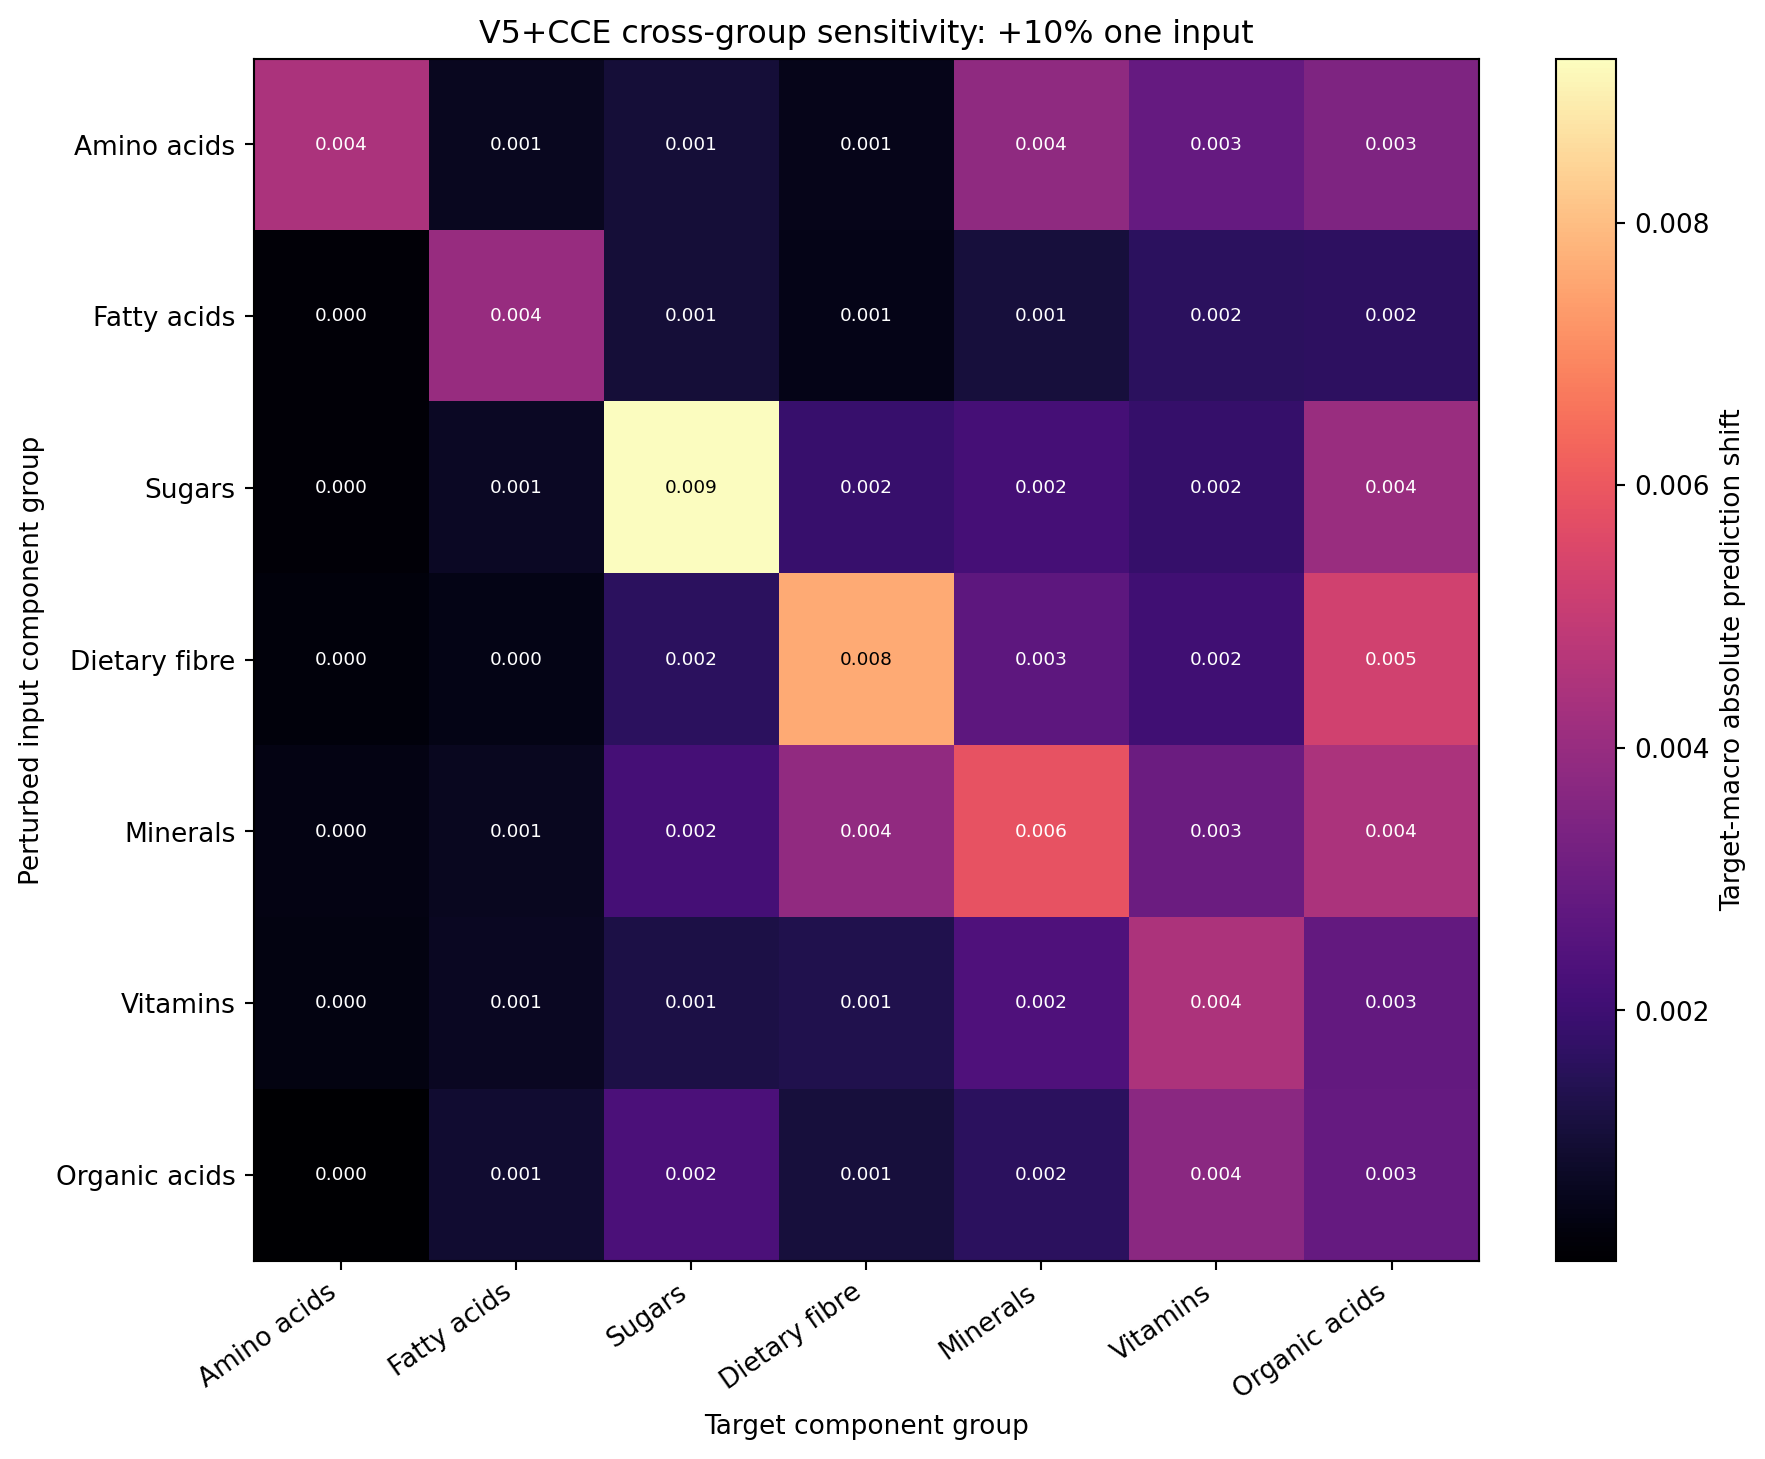
\includegraphics[width=0.76\textwidth]{group_sensitivity_plus10.png}
\caption{V5+CCE prediction shift after increasing one visible input by 10\%.}
\label{fig:group-plus}
\end{figure}

\begin{figure}[H]
\centering
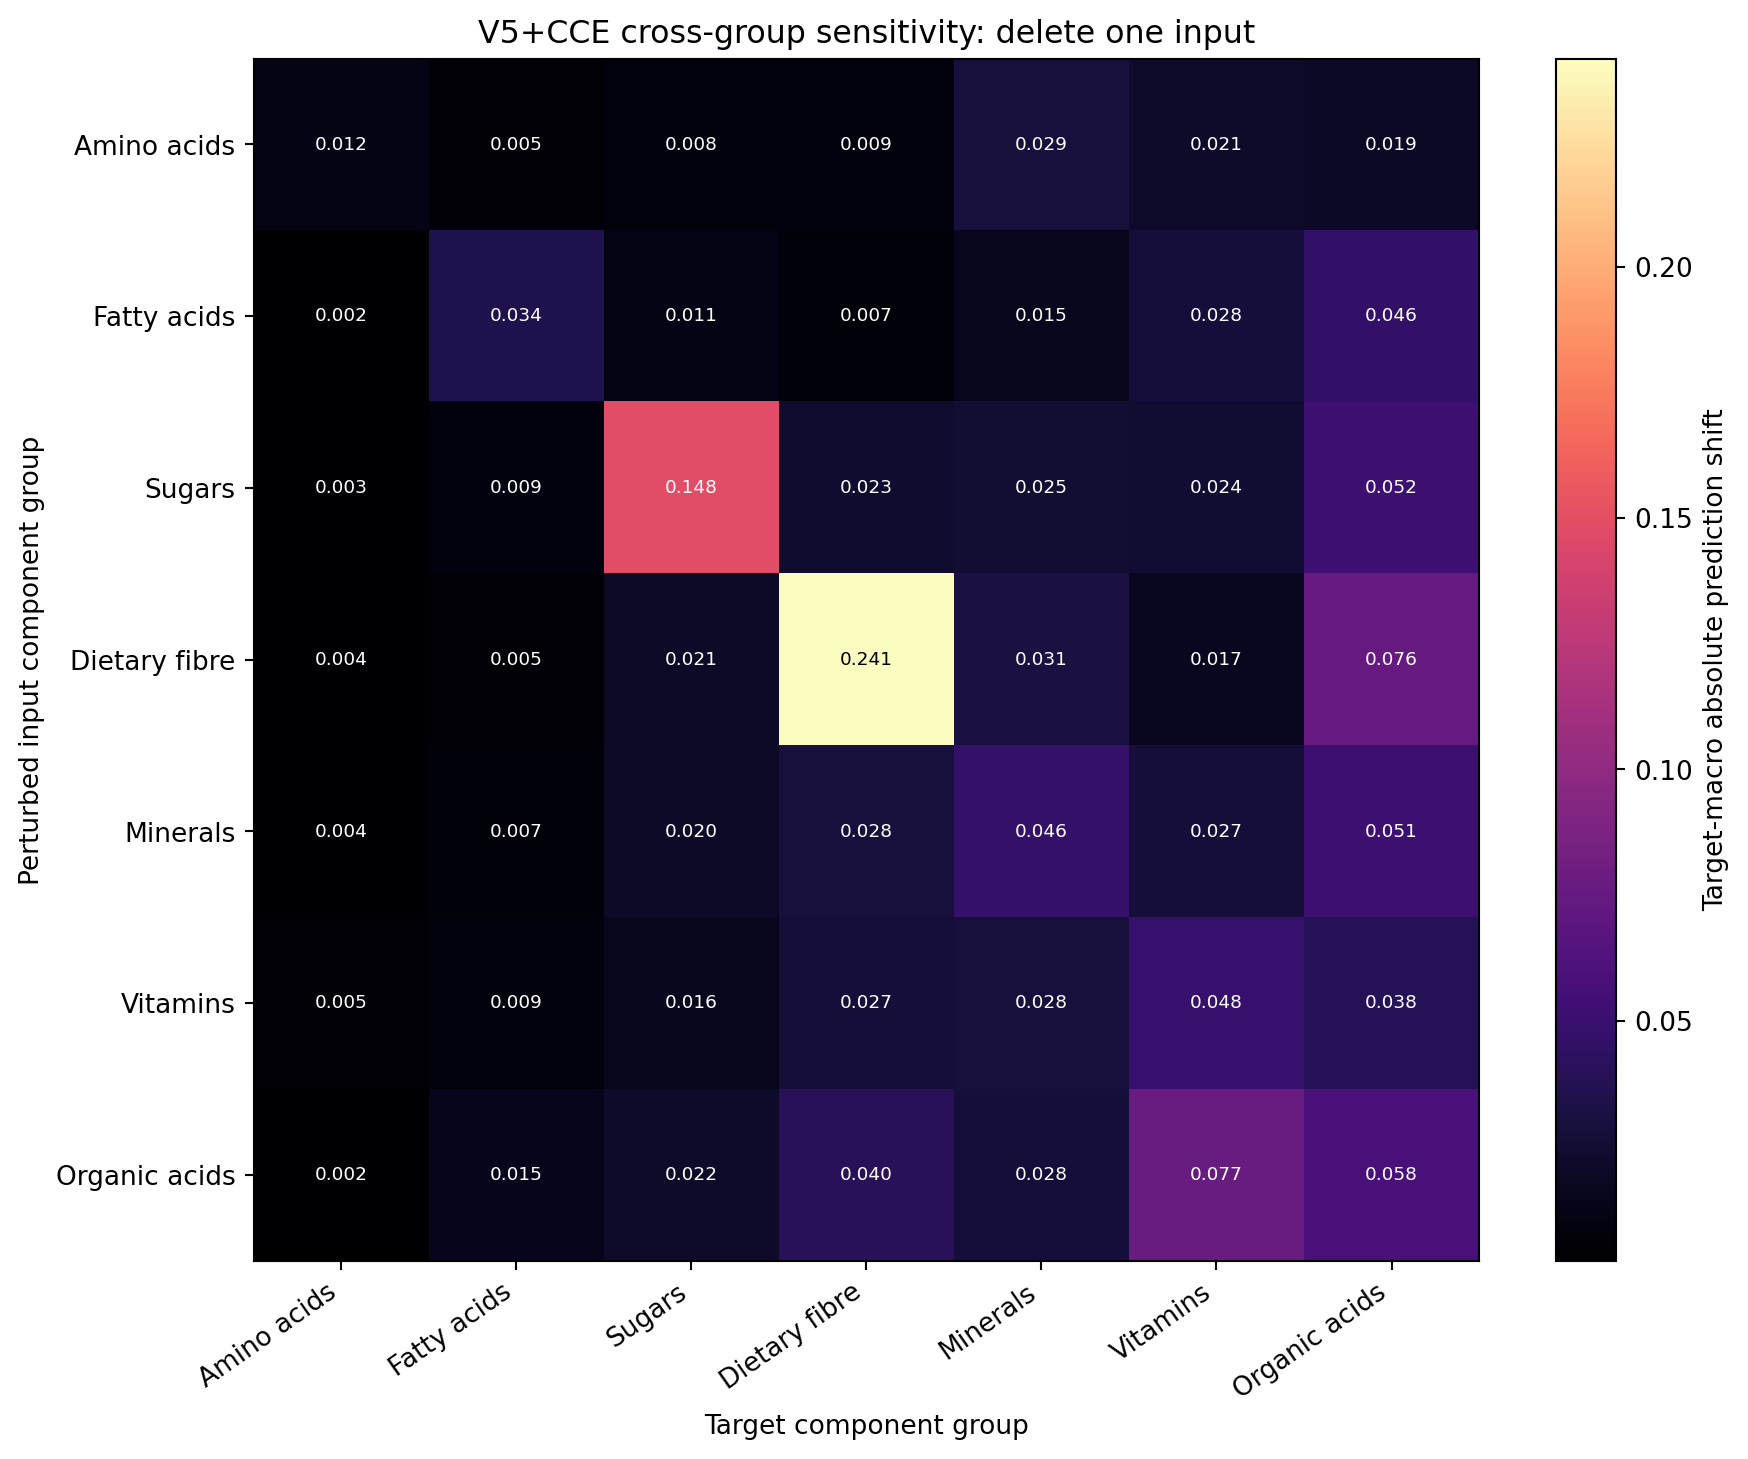
\includegraphics[width=0.76\textwidth]{group_sensitivity_deletion.png}
\caption{V5+CCE prediction shift after deleting one visible input.}
\label{fig:group-delete}
\end{figure}

\begin{table}[H]
\centering
\caption{Within-group and between-group sensitivity.}
\begin{tabular}{@{}llrrr@{}}
\toprule
Condition & Relation & Prediction shift & Error change & Pairs \\
\midrule
$-10\%$ & Between group & 0.00197 & $-0.00024$ & 45,269 \\
$-10\%$ & Within group & 0.00609 & $-0.00016$ & 12,928 \\
$+10\%$ & Between group & 0.00179 & 0.00024 & 45,269 \\
$+10\%$ & Within group & 0.00550 & 0.00097 & 12,928 \\
Deletion & Between group & 0.02230 & 0.00134 & 45,269 \\
Deletion & Within group & 0.08410 & 0.03492 & 12,928 \\
\bottomrule
\end{tabular}
\end{table}

The average diagonal response is approximately 3.1 times the off-diagonal mean for $+10\%$ and 3.8 times for deletion. Sugars and dietary fibre have the largest diagonal cells, although some dietary-fibre cells have low support. These measurements establish predictive association within the model, not causal nutritional effects.

\FloatBarrier
\section{Dependency-Family Exposure and Perturbation Ablation}

This ablation uses only target-specific ancestors or descendants that the policy normally hides; siblings are already visible. It covers 6,889 jobs, 32 targets, and five registered dependency components. Starting from the standard masked input, it exposes one, half, or all observed relatives.

\begin{figure}[H]
\centering
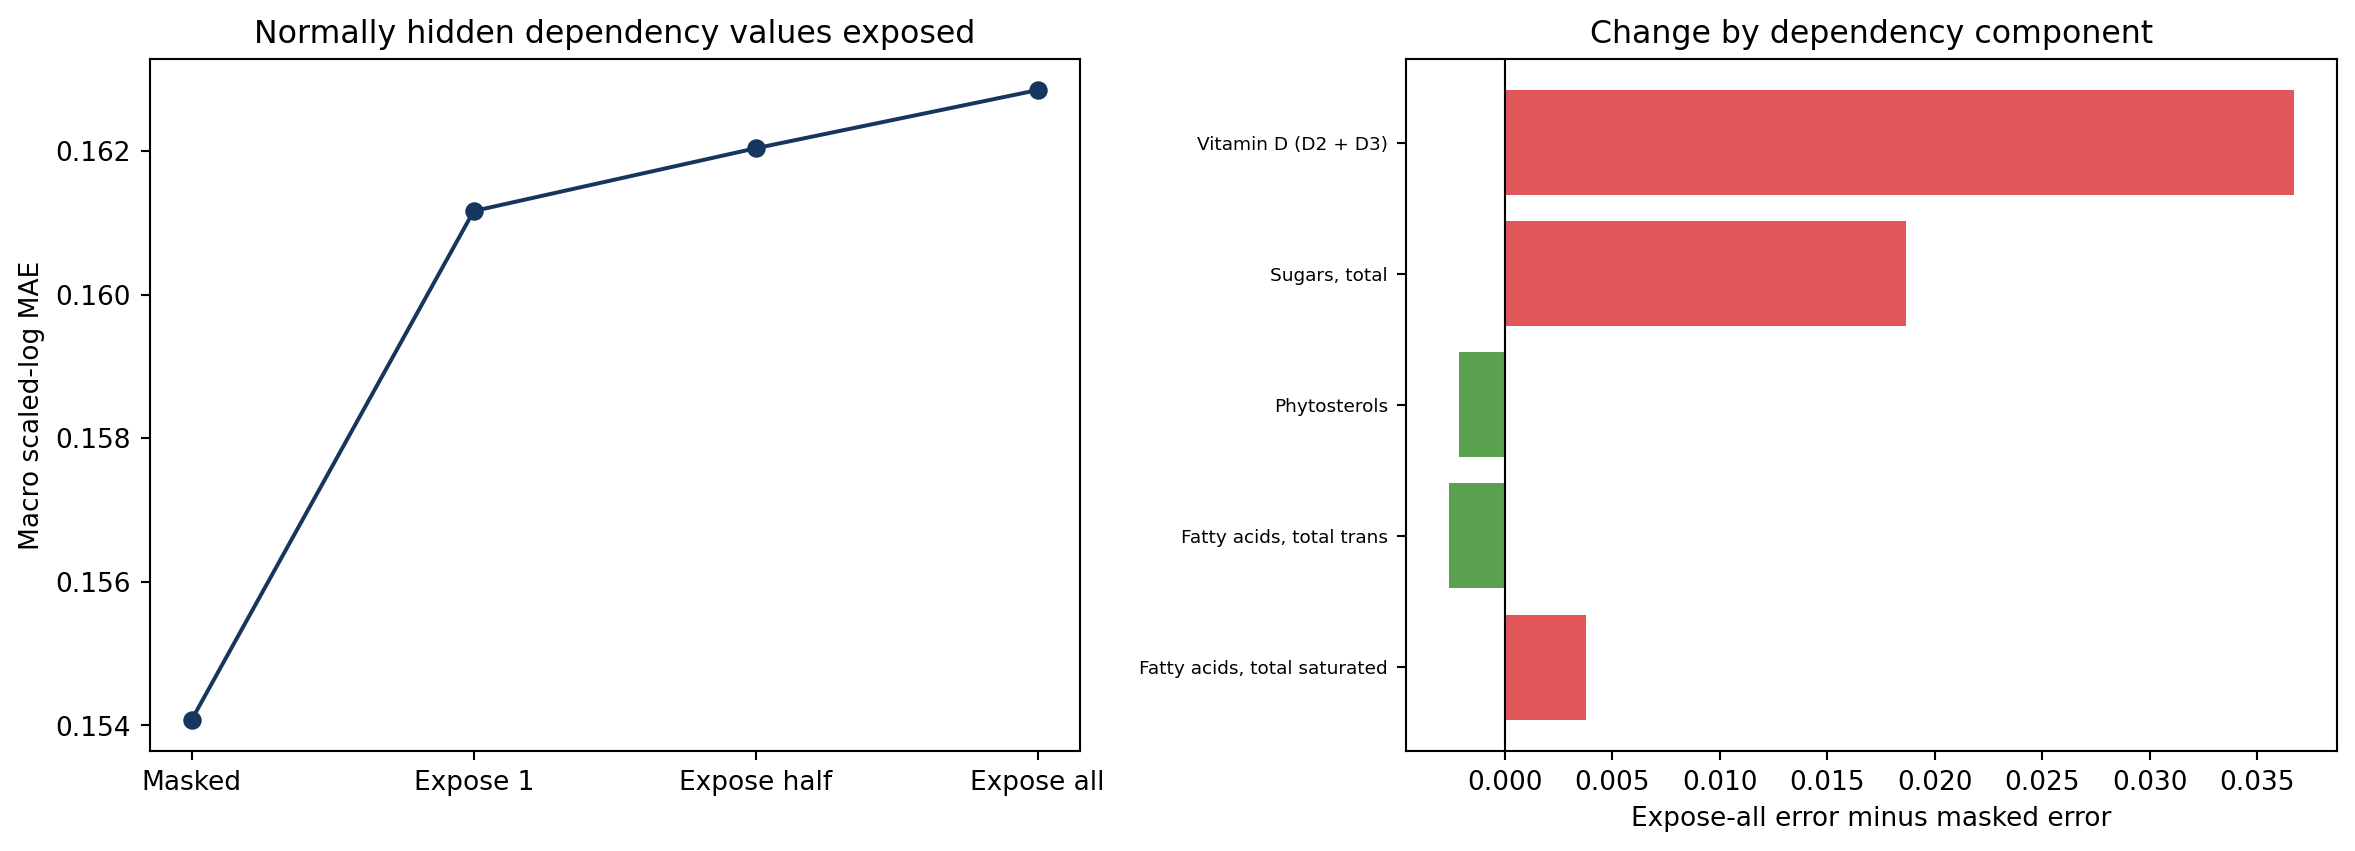
\includegraphics[width=0.92\textwidth]{dependency_exposure_ablation.png}
\caption{Accuracy and component-level change as normally hidden dependency values are exposed.}
\label{fig:dep-expose}
\end{figure}

\begin{table}[H]
\centering
\caption{Overall dependency-exposure ablation.}
\begin{tabular}{@{}lrrrr@{}}
\toprule
Condition & Scaled-log MAE & Shift vs. masked & Axes & Jobs \\
\midrule
Standard mask & \textbf{0.1541} & 0.0000 & 32 & 6,889 \\
Expose one relative & 0.1612 & 0.0237 & 32 & 6,889 \\
Expose half & 0.1620 & 0.0256 & 32 & 6,889 \\
Expose all & 0.1628 & 0.0290 & 32 & 6,889 \\
\bottomrule
\end{tabular}
\end{table}

Exposing more dependency values does not improve accuracy. This is an out-of-distribution inference condition: training never presents a task in which the target is simultaneously visible to its registered ancestors or descendants.

One exposed dependency value is then compared with a visible non-dependency control matched by INFOODS group and normalized-value proximity. Each is perturbed separately.

\begin{figure}[H]
\centering
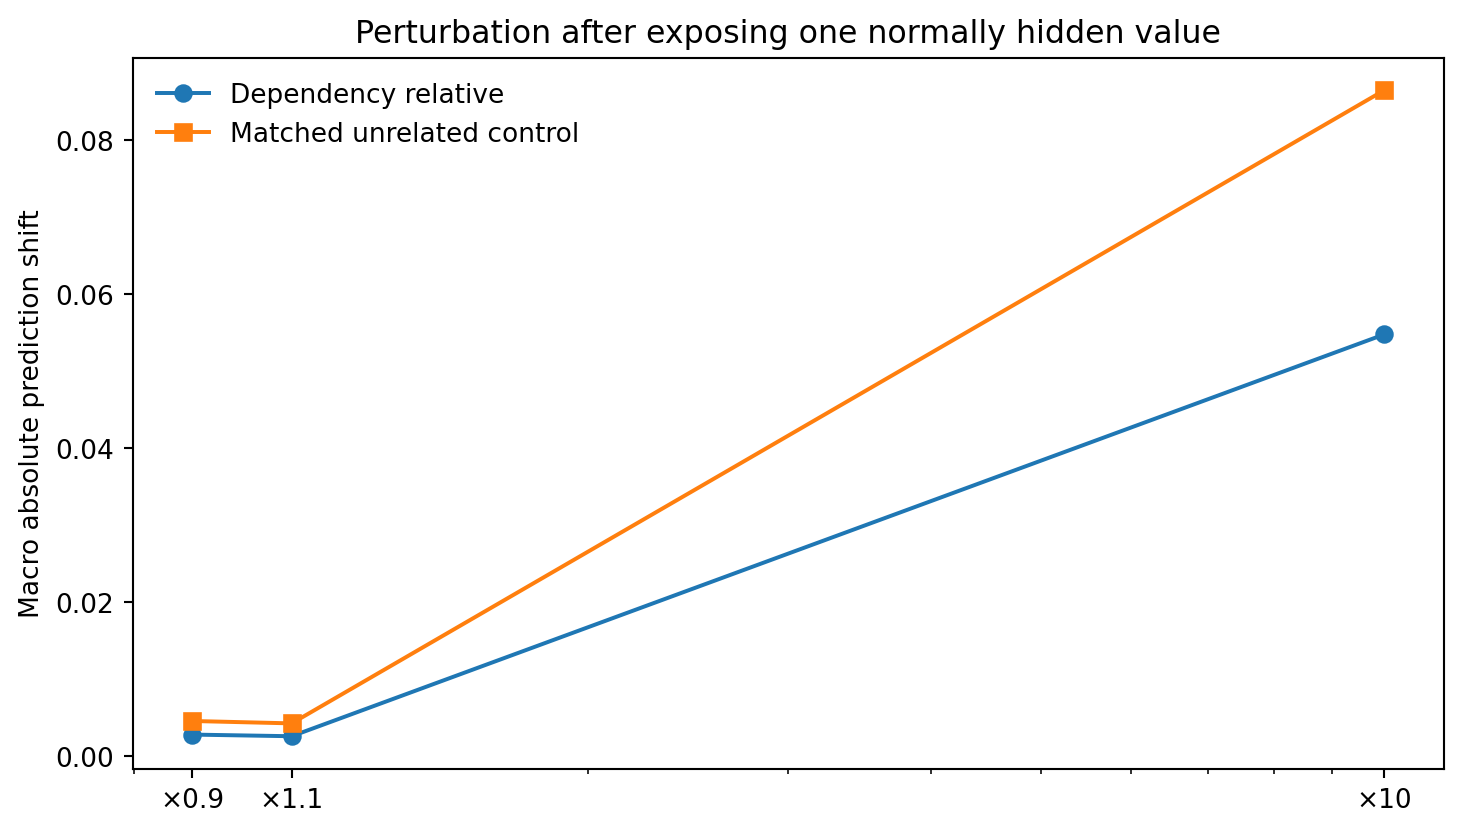
\includegraphics[width=0.82\textwidth]{dependency_perturbation_ablation.png}
\caption{Prediction shift after perturbing one exposed dependency value or its matched unrelated control.}
\label{fig:dep-perturb}
\end{figure}

\begin{table}[H]
\centering
\caption{Dependency-relative versus matched-control perturbation.}
\begin{tabular}{@{}rrrrr@{}}
\toprule
Factor & Dependency shift & Control shift & Dependency $\Delta$error & Control $\Delta$error \\
\midrule
0.9 & 0.0028 & 0.0046 & $-0.0007$ & 0.0003 \\
1.1 & 0.0026 & 0.0042 & 0.0007 & 0.0004 \\
10.0 & 0.0548 & 0.0865 & 0.0177 & 0.0400 \\
\bottomrule
\end{tabular}
\end{table}

Revealing one dependency relative shifts predictions by 0.02371, compared with 0.02991 for a matched visible control. The profile-bootstrap 95\% interval for dependency minus control is $[-0.01124,0.00091]$ and crosses zero. Across all three value perturbations, dependency-relative shifts are also smaller than control shifts. The ablation therefore does not show that the current model relies more heavily on strict dependency relatives than on ordinary inputs. Its defensible conclusion is narrower: inference-only unmasking changes predictions and worsens aggregate error, so it should not replace the training-time mask. Measuring leakage from omitting the mask would require a separately trained, matched no-dependency-mask model.

\section{Conclusions and Limitations}

\begin{enumerate}
  \item The explicit dependency mask is part of training and every evaluation path; it is not an inference-only adjustment.
  \item V5+CCE has the best complete-test and strict Taiwan zero-shot scaled-log MAE among the formal methods in this study.
  \item Frozen V5+CCE remains better than Taiwan-only RF and XGBoost fits at 8, 32, and 128 profiles, providing evidence of external sample efficiency from source pretraining.
  \item V5+CCE is strongest with 5--20 visible composition values; tree models regain the advantage when context is more complete.
  \item FAO/INFOODS group sensitivity is larger within registered broad component groups on average, but this is a model association audit rather than a causal analysis.
  \item The strict dependency exposure experiment is a negative result: it supports keeping the mask but does not demonstrate unusually strong learned parent--component reliance.
\end{enumerate}

Taiwan covers only 80 of 187 supervised targets. Food-name novelty does not guarantee complete semantic novelty. Database clusters in UMAP are strongly confounded by missingness and coverage. The neural results come from one pretrained seed. The Taiwan few-shot comparison intentionally gives pretraining only to V5+CCE, so it demonstrates the value of the pretrained system as deployed rather than an architecture-controlled pretraining comparison.

\section{Reproducibility Package}

This directory is self-contained for report review. It includes this \LaTeX{} source, the compiled PDF, all eight figures referenced above, and 18 aggregate CSV files in \path{tables/}. The CSVs contain model-level, per-condition, or bootstrap summaries only. No checkpoint, raw database, Taiwan source file, derived profile matrix, or row-level prediction is included.

\begin{thebibliography}{9}

\bibitem{infoodsworkshop}
FAO/INFOODS and EuroFIR.
\newblock Report of the 9th International Food Data Conference and component nomenclature workshop, Annex 1: draft INFOODS component hierarchy.
\newblock \url{https://www.fao.org/fileadmin/templates/food_composition/documents/upload/9IFDCReportfinal.pdf}

\bibitem{infoodstags}
FAO/INFOODS.
\newblock Food component identifiers (tagnames), standards and guidelines.
\newblock \url{https://www.fao.org/infoods/infoods/standards-guidelines/food-component-identifiers-tagnames/en/}

\bibitem{scgpt}
H. Cui, C. Wang, H. Maan, et al.
\newblock scGPT: Toward building a foundation model for single-cell multi-omics using generative AI.
\newblock \emph{Nature Methods}, 21:1470--1480, 2024.
\newblock \url{https://doi.org/10.1038/s41592-024-02201-0}

\bibitem{umap}
L. McInnes, J. Healy, and J. Melville.
\newblock UMAP: Uniform manifold approximation and projection for dimension reduction.
\newblock arXiv:1802.03426, 2018.
\newblock \url{https://arxiv.org/abs/1802.03426}

\end{thebibliography}

\end{document}
